\section{Experiments}
\label{section:experiments}

For consiceness, several experiments are relagated in appendix: 

\begin{enumerate}
    \item \textbf{TS-LDDMM representation identifiability, \Cref{appendix:identifiability}:} On synthetic data, we evaluate the ability of our method to retrieve the parameter $v_0^*$ that encodes the deformation $\varphi^{\{v_0^*\}}$ acting on a time series graph $\msg$ by solving the geodesic shooting problem \eqref{eq:relaxation} between $\msg$ and $\varphi^{\{v_0^*\}}.\msg$. \textbf{Results} show that TS-LDDMM representations are identifiable or weakly identifiable depending on the velocity field kernel $K_G$ specification.
  
    \item \textbf{Robustness to irregular sampling} We compare the robustness of TS-LDDMM representation with 9 URL methods handling irregularly sampled multivariate time series on 15 shape-based datasets (7 univariates \& 8 multivariates). We assess methods' classification performances under regular sampling (0\% missing rate) and three irregular sampling regimes (30\%, 50\%, and 70\% missing rates), according to the protocol depicted in \cite{kidger2020neural}. \textbf{Results} show that our method, TS-LDDMM, outperforms all methods for sampling regimes with missing rates: 0\%, 30\%, and 50\%. The performance decrease of the Kernel-SVC based on TS-LDDMM representation is sensibly due to the misspecification of its regularization parameter.
    
    \item \textbf{Classification benchmark on regularly sampled datasets, \Cref{appendix:classification_shape_analysis}:} We compare performances of a kernel support vector machine (SVC) algorithm based on TS-LDDMM representation with 3 state-of-the-art classification methods from shape analysis on 15 shape-based datasets (7 univariates \& 8 multivariates). \textbf{Results} show that the TS-LDDMM-based method outperforms other methods (best performances over 13 datasets), making TS-LDDMM representation relevant for time series shape analysis.
\end{enumerate}


\subsection{Interpretability: analysis of respiratory behavior in mice}
%We consider a dataset composed of mouse respiratory time series before and after a drug injection.
% A complete presentation of this dataset is given in \Cref{appendix:mouse_dataset}.
%  The mouse are divided in two groups depending on their genotypes : \textit{colq} and \textit{wt}.
%  We aim to study the difference of respiratory shapes according to the genotype.
%   That is why, TS-LDDMM \eqref{eq:general_optimization_problem} is applied to derive the features representations $(\mathbf{\alpha}_j)_{j\in[N]}\in (\Rset^2)^N$ related to $N$=\sam{fill} respiratory time series coming from 14 mouse (7 \textit{colq} and \textit{wt}) before drug injection.
%   Then, a Principal Components Analysis (PCA) is performed on $(\mathbf{\alpha}_j)_{j\in[N]}$
\begin{figure*}[t]
  \centering
  \begin{subfigure}[b]{0.49\textwidth}
    \centering
    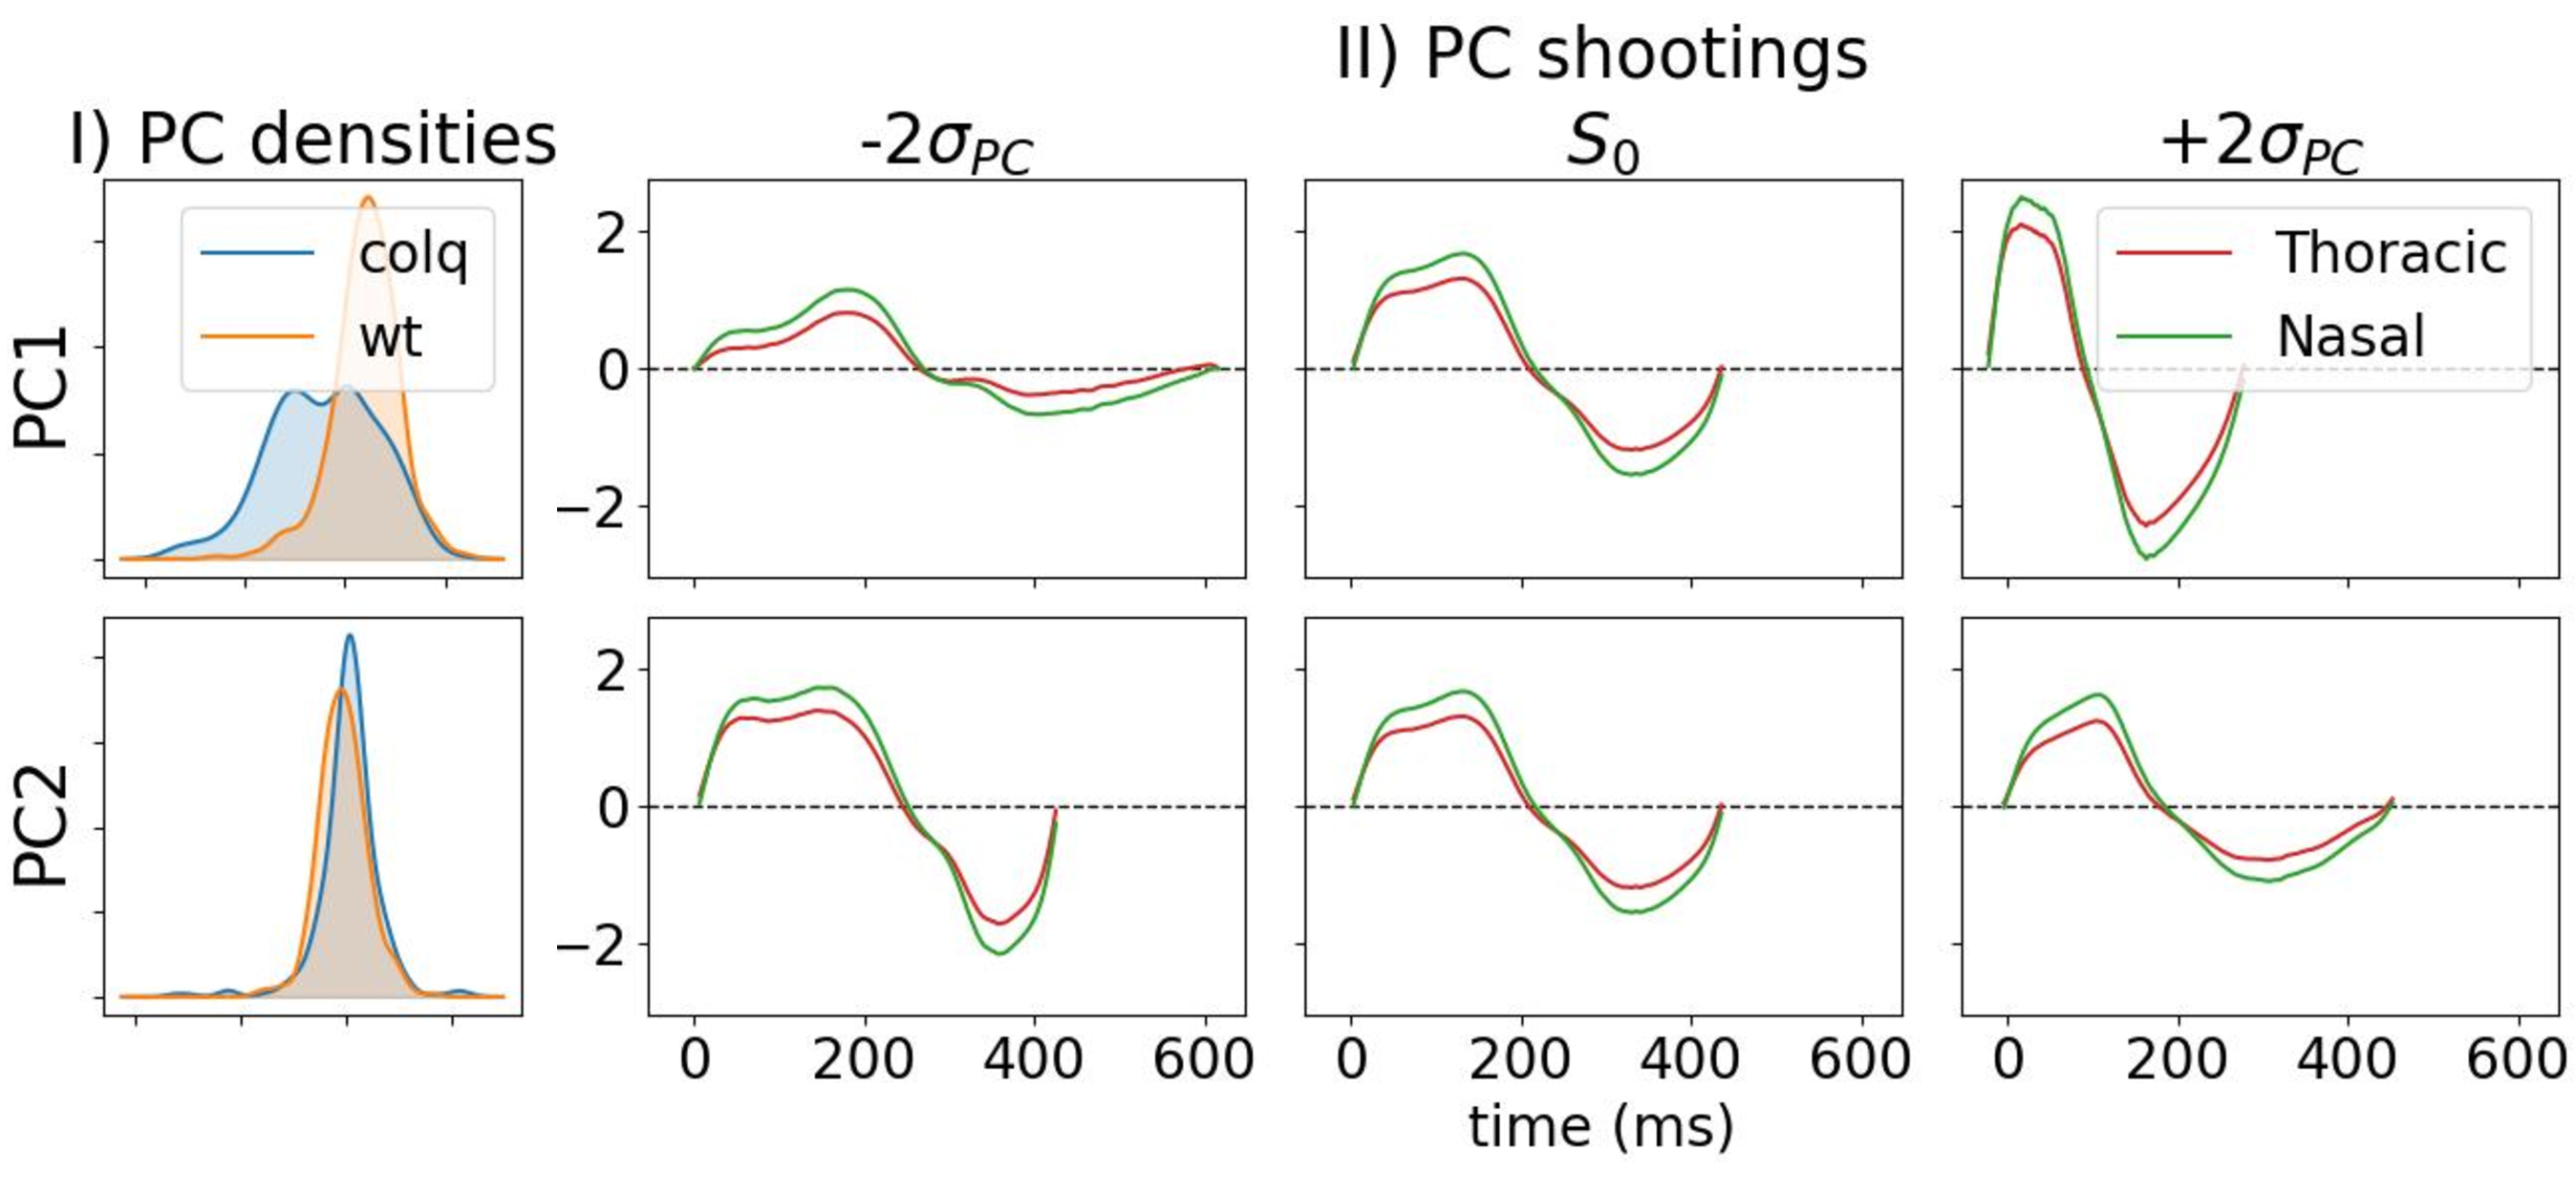
\includegraphics[width = \textwidth]{pictures/ts_ddmm_shooting.pdf}
    \caption{TS-LDDMM}
    \label{fig:ts-lddmm shooting}
  \end{subfigure}
  \begin{subfigure}[b]{0.49\textwidth}
    \centering
    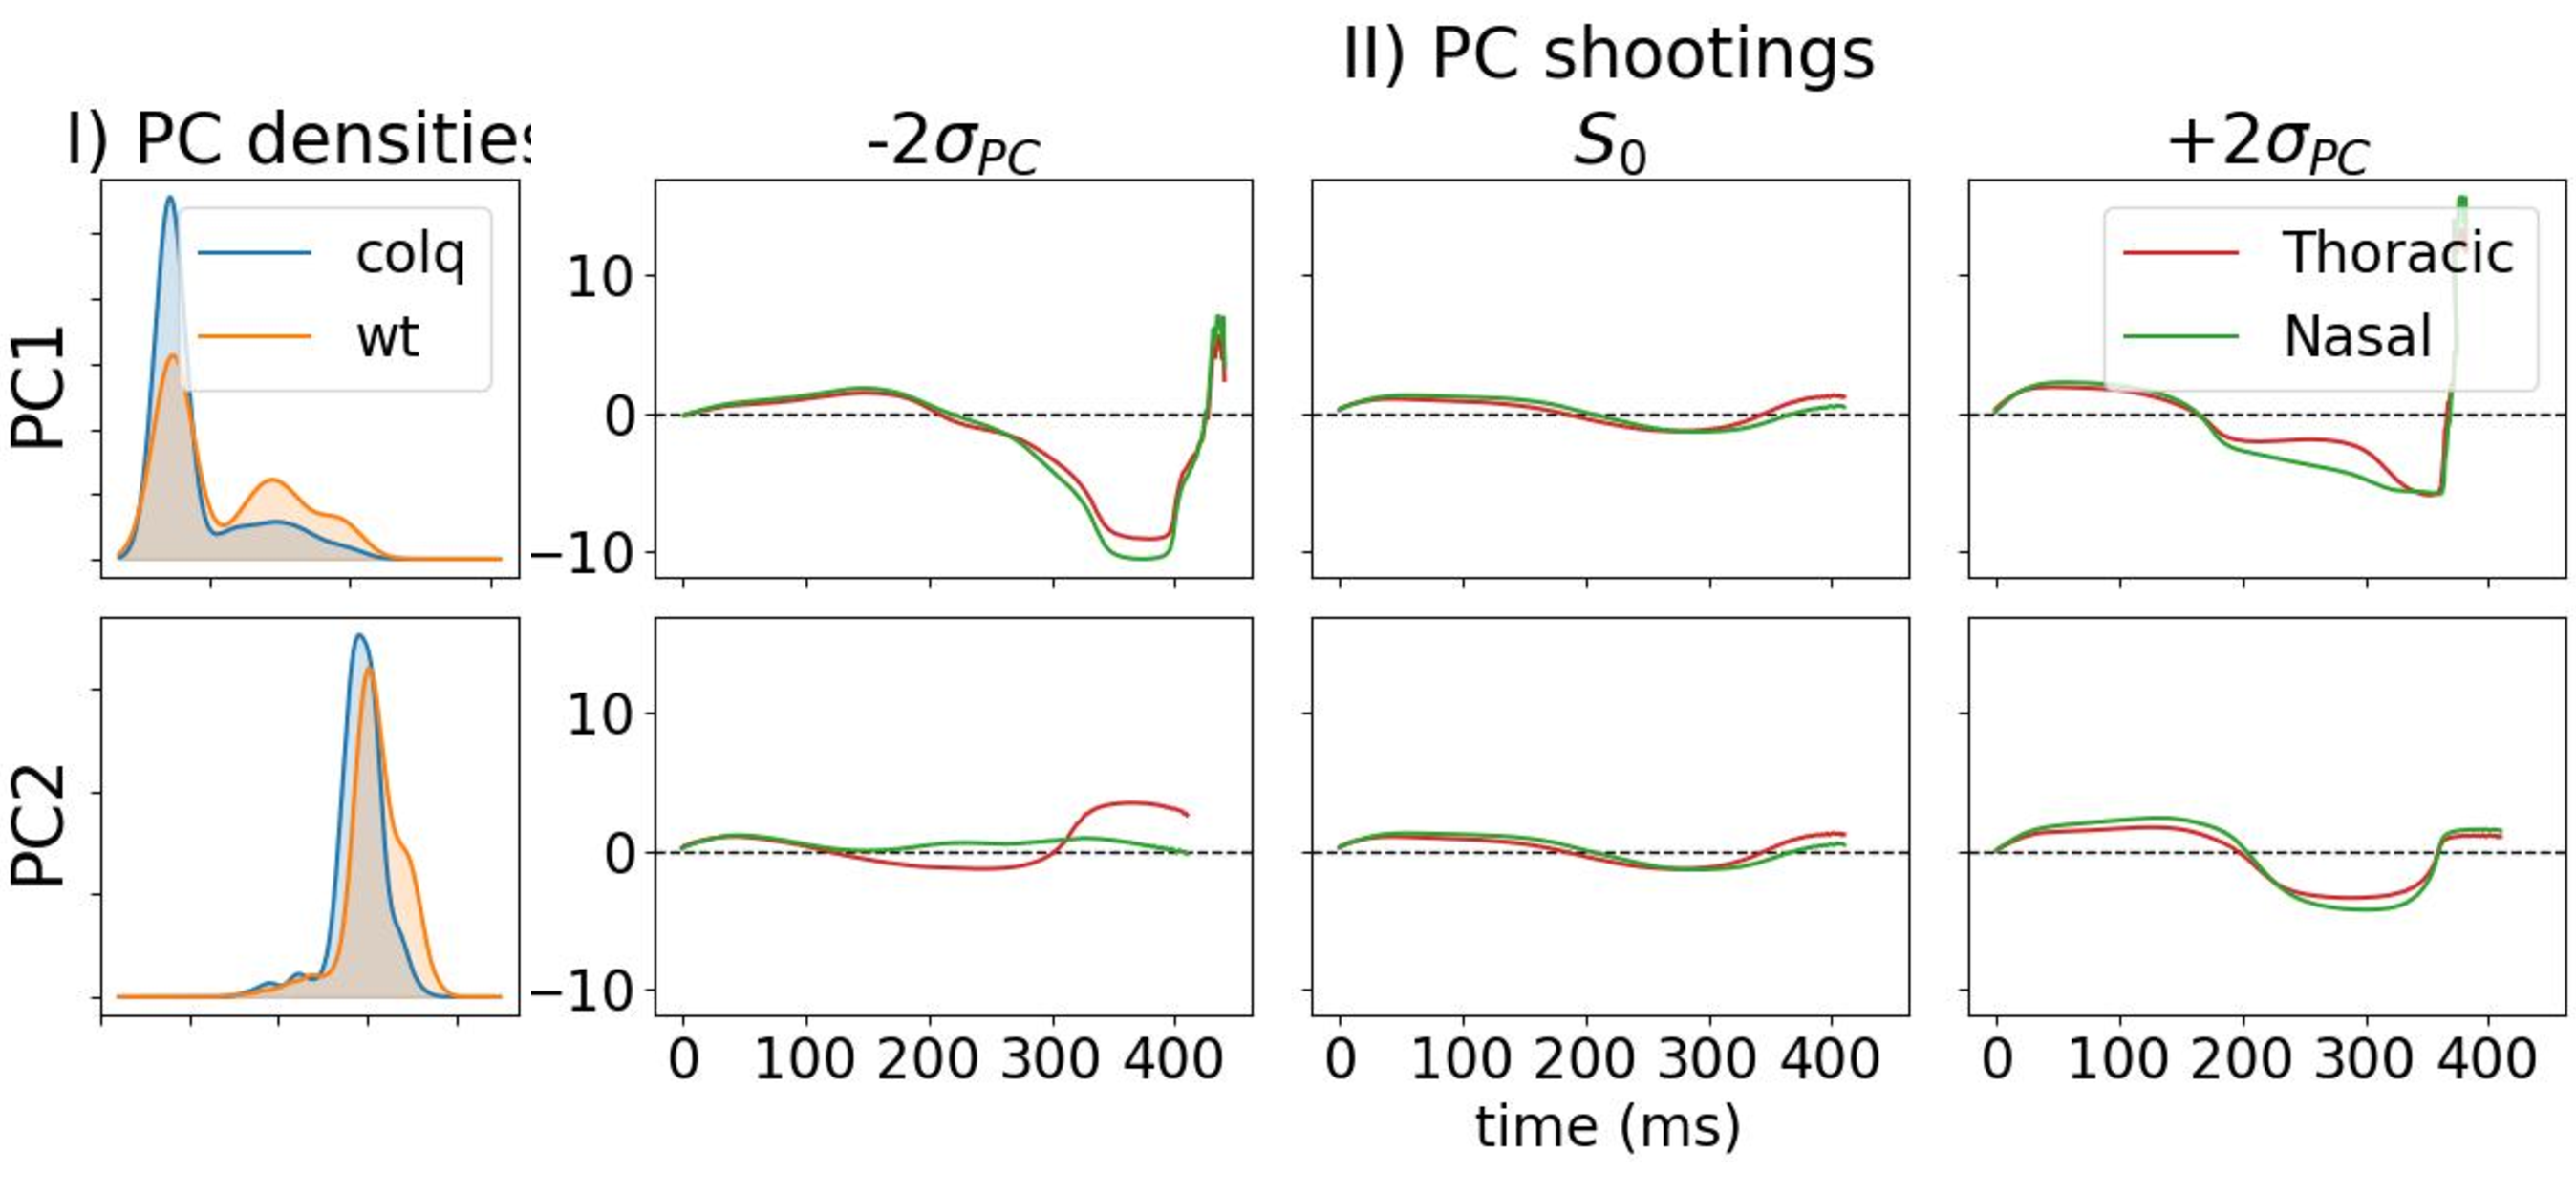
\includegraphics[width = \textwidth]{pictures/lddmm_shooting.pdf}
    \caption{LDDMM}
    \label{fig:lddmm shooting}
  \end{subfigure}
  \caption{Analysis of the two principal components (PC) related to mice' respiratory cycles before exposure for TS-LDDMM \Cref{fig:ts-lddmm shooting}, and LDDMM \Cref{fig:lddmm shooting}.
  In both cases, I) displays PC densities according to mice genotype and II) displays  deformations of the reference graph $S_0$ along each PC.}
\end{figure*}

\begin{wrapfigure}{r}{0.50\textwidth}
  \centering
  \begin{subfigure}[b]{0.16\textwidth}
    \centering
    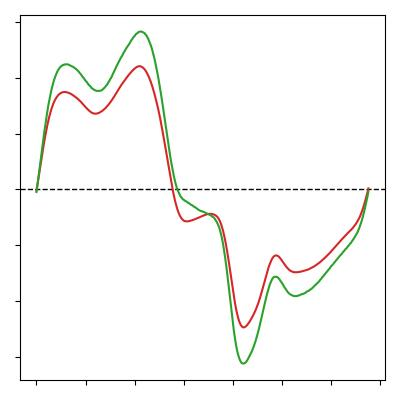
\includegraphics[width = \textwidth]{pictures/exp_1_cycle_example.jpeg}
    \caption{Colq cycle}
    \label{fig:colq-cycle}
  \end{subfigure}
  \begin{subfigure}[b]{0.16\textwidth}
    \centering
    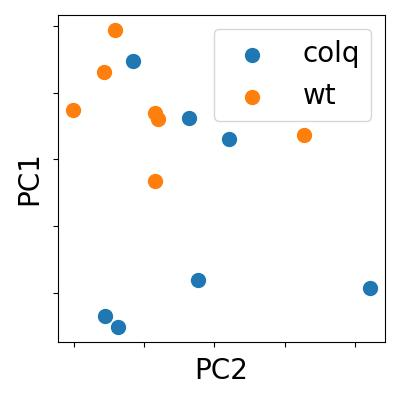
\includegraphics[width = \textwidth]{pictures/exp_1_scatter.jpeg}
    \caption{PC1 vs PC2}
    \label{fig: pcs-scatter}
  \end{subfigure}
  \begin{subfigure}[b]{0.16\textwidth}
    \centering
    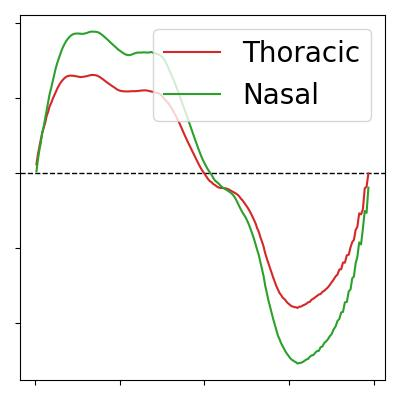
\includegraphics[width = \textwidth]{pictures/exp_1_barycenter.jpeg}
    \caption{WT reference}
    \label{fig:wt-reference}
  \end{subfigure}
  \caption{\Cref{fig:colq-cycle} is a \textbf{colq} respiratory cycle. \Cref*{fig: pcs-scatter} displays individual mouse reference respiratory cycle in the TS-LDDMM PC1-PC2 coordinates. \Cref{fig:wt-reference} is a referent respiratory cycle of a \textbf{wt} mouse learned with TS-LDDMM. }
\end{wrapfigure}


%the densities of each genotype according to each PC are displayed. In Figure B), the deformations of the reference graph $S_0$ along each PC are given. In Figure D), the graph of reference $S^j$, also called barycenter, related to each mouse, is displayed according to their coordinates on PC1 and PC3. In Figure C) et E), illustrations of respiratory cycles related to mice coming from the \textbf{wt} and \textbf{colq} group are displayed.

%\begin{figure*}[t]
%  \centering
%  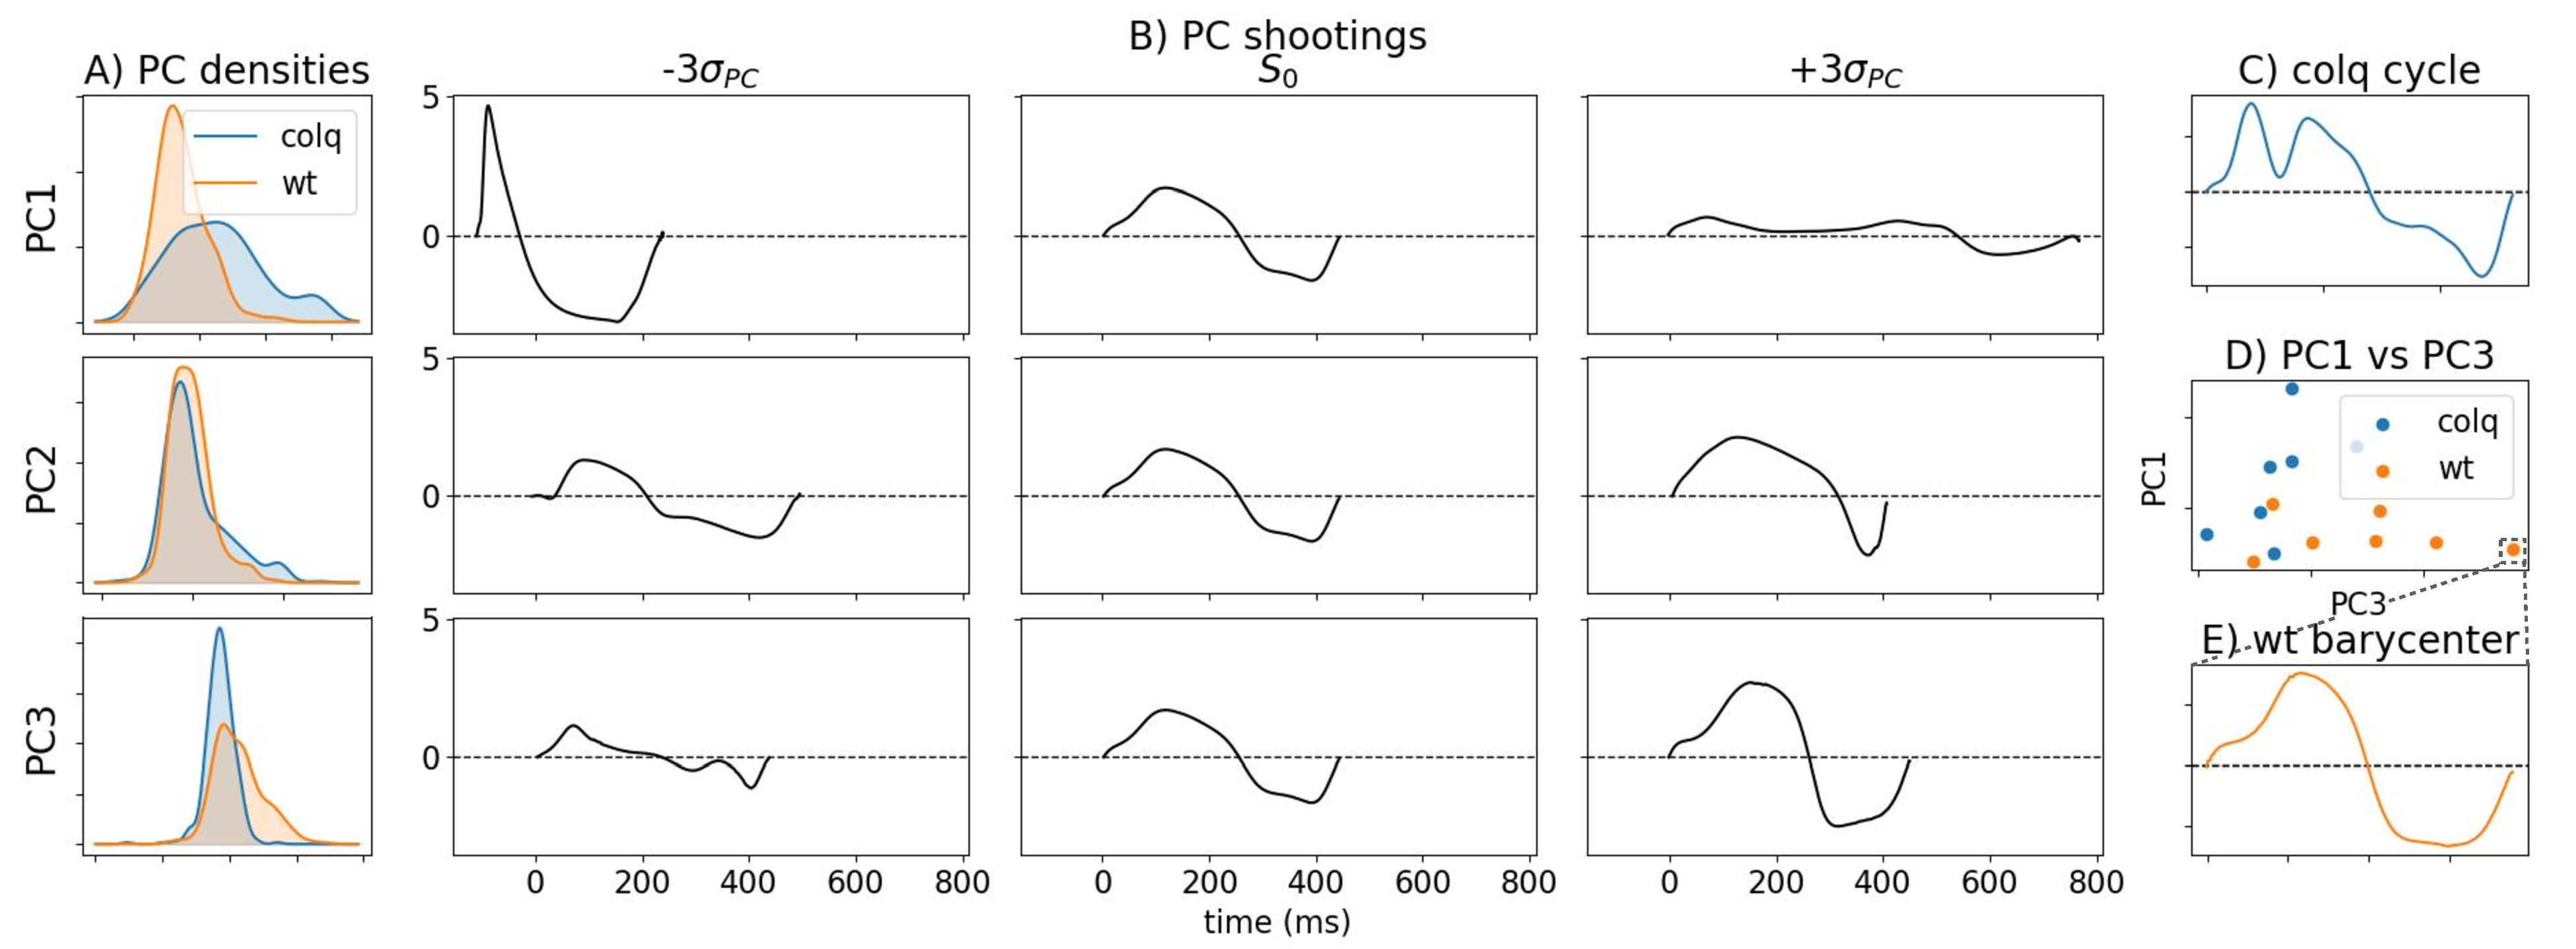
\includegraphics[width=0.95\linewidth]{"./pictures/exp_1_bis.pdf"}
%  \vspace{-1.5em}
%  \caption{Analysis of the two principal components (PC) related to the mice respiratory cycles before exposure for TS-LDDMM \Cref{fig:ts-lddmm shooting}.
%  In Figure A), the densities of each genotype according to each PC are displayed. In Figure B), the deformations of the reference graph $S_0$ along each PC are given. In Figure D), the graph of reference $S^j$, also called barycenter, related to each mouse, is displayed according to their coordinates on PC1 and PC3. In Figure C) et E), illustrations of respiratory cycles related to mice coming from the \textbf{wt} and \textbf{colq} group are displayed.  }
%  \label{fig:exp_1_PCA}
%  %\vspace{-1em}
%\end{figure*}

This experiment highlights the \textit{interpretability} of TS-LDDMM representation for studying the inter-individual variability in time series biomedical datasets. We consider a multivariate time series dataset that accounts for mice's nasal and thoracic airflow evolution when exposed to an irritant molecule altering respiratory functions \cite{nervo2019respiratory}.
The dataset is divided into two groups, one composed of 7 control mice (\textbf{wt}) and the other of 7 mice (\textbf{colq}) deficient in an enzyme involved in the control of respiration. For each mouse, airflows were recorded for 15 to 20 minutes before exposure to the irritant molecule and then for 35 to 40 minutes. A complete 
description of the dataset is given in the \Cref{appendix:mouse_dataset}.

\paragraph{Result summary:} By comparing the shape of individual respiratory cycles (inspiration + expiration, see \Cref{fig:exp_1_PCA}-C), we show that TS-LDDMM features can encode genotype distinctive breathing behaviors and their evolution after exposure to the irritant molecule. 

\paragraph{Breathing behaviors before exposure} We first compare breathing behaviors before exposure.
Solving \eqref{eq:general_optimization_problem}, we derive the reference respiratory cycle's graph $S_0$ and the TS-LDDMM features representations 
$(\alpha_j)_{j\in[N_1]}$ related to $N_1=700$ respiratory cycles extracted according 
to the procedure \cite{germain2023unsupervised}.
Then, we perform a kernel PCA on the initial velocity field $\left(v_0(\alpha_j,S_0)\right)_{j\in[N_1]}\in \msv^{N_1}$ defined in \eqref{eq:def_v0}.
In \Cref{fig:exp_1_PCA}, we focus on the analysis of the three Principal Components (PC).

As observable from \Cref{fig:exp_1_PCA}-B), principal components refer to different types of deformations. 
By interpreting \Cref{fig:exp_1_PCA}-B): Only PC1 accounts for time warping, PC2 expresses the trade-off between inspiration and expiration duration, and PC3 corresponds to a change in signal amplitude.
 Compared to \textbf{wt} mice, the distribution of \textbf{colq} mice 
TS-LDMMM feature representation along the PC1 axis has a heavy tail and the associated deformation (+3 $\sigma_{\text{PC}}$) 
shows an inspiration with two peaks. As illustrated in \Cref{fig:exp_1_PCA}-A), such respiratory cycles are preponderant
 with \textbf{colq} mice and may be caused by motor impairment due to their enzyme deficiency, \cite{germain2023unsupervised}.
  In addition, 
 the \textbf{colq} mice were smaller than the \textbf{wt} mice due to a delay in growth caused by their lack of an enzyme. 
 This difference can be seen on PC3 since the volumes of air (area under the curve) inspired and exhaled are
  smaller for the smaller mice. In correlation, the distribution of \textbf{wt} mice TS-LDDMM feature representations 
  along the PC3 axis have a heavy tail corresponding to large air volume as depicted by the deformation 
  (+3 $\sigma_{\text{PC}}$) in \Cref{fig:exp_1_PCA}-B). Finally, \Cref{fig:exp_1_PCA}-D) shows that PC1 and PC3 capture the main differences between
   the two groups as their respective reference graphs $S^j$ are located in different parts of the space. 
%In Figure \Cref{fig:exp_1_PCA}, we display coordinates densities per genotype and PC.
\begin{figure*}[t]
  \centering
  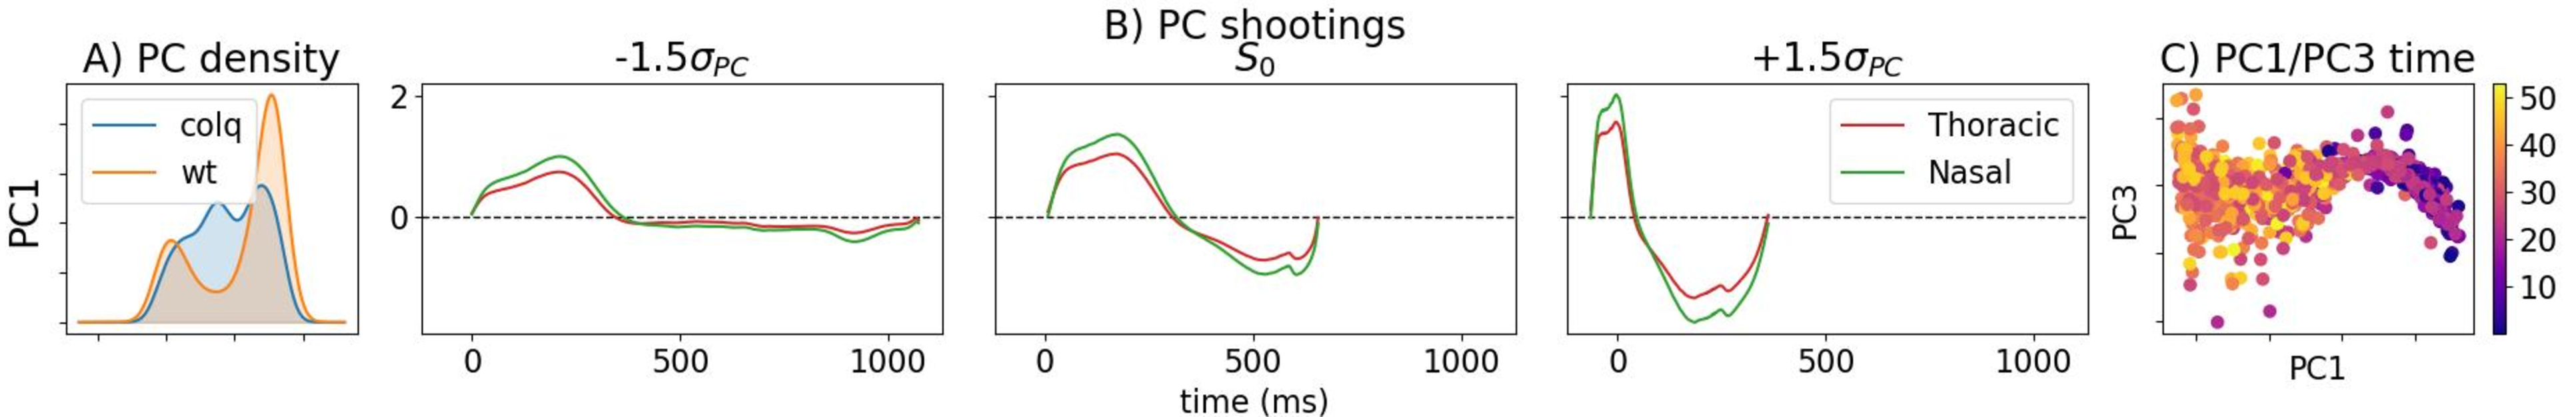
\includegraphics[width=0.95\linewidth]{"./pictures/exp2.pdf"}
  \caption{Analysis of the first Principal Component (PC1) related to mice' respiratory cycles before and after exposure for TS-LDDMM. Figure A) displays PC densities according to mice genotype, Figure B) displays  deformations of the reference graph $S_0$ along PC1, and Figure C) displays respiratory cycles with respect to time in PC1 and PC3 coordinates}
  \label{fig:exp_2_PCA}
  \vspace{-1.5em}
\end{figure*}
We perform a second experiment to analyze the evolution of breathing behaviors when mice are exposed to the irritant 
molecule. We follow the same procedure as before. However, we take $N_2=1400$ with 25\% (resp. 75\%) 
before (resp. after) exposure. In \Cref{fig:exp_2_PCA}, we focus on the first principal component PC since
it encodes the effect of the irritant molecule as depicted in \Cref{fig:exp_2_PCA}-C) (the exposure occurs at 20 minutes).
\Cref{fig:exp_2_PCA}-B) shows that the deformation (+3 $\sigma_{\text{PC}}$) leads to longer respiratory cycles that include pauses,
as observed in \cite{germain2023unsupervised}. As well, \Cref{fig:exp_2_PCA}-A) shows that TS-LDDMM features distributions are less spread 
out for \textbf{colq} mice compared to \textbf{wt} mice. Indeed, the irritant molecule inhibits the action of the 
deficient enzyme, \textbf{wt} mice strongly react to the irritant molecule, whereas \textbf{colq} mice are better 
adapted due to their deficiency.
%Secondly, we compare breathing behaviors before and after exposure to observe the impact of the irritant molecule.
% We follow the same procedure as for before exposure, but we take $N_2=1400$ respiratory cycles extracted according 
% to the procedure CITE....
% In \Cref{fig:exp_2_PCA}, we focus on the first Principal Component (PC) since it encodes the effect of the irritant molecule as demonstrated on Figure \ref{fig:exp_2_PCA}-C) (exposure at time 20).
% We observe on \Cref{fig:exp_2_PCA}-B) that after exposure the mouse have longuer breath such that the expiration is longuer than inspiration.
%  Moreover, we deduce from Figure \ref{fig:exp_2_PCA}-A) that \textbf{colq} are more constant in their breath compared to \textbf{wt} after exposure.
%
% In Figure REF, we 
% also display the reference respiratory cycle S0 and its deformations in the principal component directions.
%  Additionally, we learn each mouse's reference respiratory cycle and represent them in the first and third PC coordinates system in Figure REF. 



\subsection{Quantitative performances of the TS-LDDMM representation in classification}
Combined with a Support Vector Classifier (SVC) \cite{hsu2003practical}, TS-LDDMM representation can be used for 
classification tasks using the kernel associated with the initial velocity space $\msv$.
We compare TS-LDDMM-SVC classification performances with another SVC using representation 
learned with T-loss \cite{franceschi2019unsupervised}, an unsupervised deep learning feature 
representation method for time series. We also include fully supervised methods in deep learning 
-ResNet, CNN \cite{ismail2019deep}- and machine learning: Catch22 \cite{lubba2019catch22}, Rocket
\cite{dempster2020rocket}, Dynamic Time Wrapping k-Nearest Neighbors (DTW-kNN) 
\cite{muller2007dynamic}. Methods are compared using f1-score on several shape-based UCR/UEA datasets 
\cite{dau2019ucr,bagnall2018uea} introduced in \Cref{appendix:classification_dataset}. All implementation details are given 
in \Cref{appendix:classification_implementation}.
\Cref{table:classification} presents the reuslts. TS-LDDMM-SVC consistently outperforms the other unsupervised methods. It is ranked 1,3,4,3 for all methods combined, 
demonstrating its competitiveness as an unsupervised method on time series dataset homogeneous regarding shape.
%TS-LDDMM representation can be used in a Support Vector Classifier (SVC) \cite{hsu2003practical} using the kernel of the space of initial velocity $\msv$.
%We compare its capacity of representation to an SVC using T-Loss representation \cite{franceschi2019unsupervised}, which is an unsupervised representation deep learning method for time series,
%and to others fully supervised methods using deep learning -ResNet, CNN \cite{ismail2019deep}- or not: Catch22 \cite{lubba2019catch22}, Rocket \cite{dempster2020rocket}, Dynamic Time Wrapping \cite{muller2007dynamic} k-Nearest Neighbors (DTW-kNN).
%These methods are compared using f1-score on several datasets introduced in \Cref{appendix:classification_dataset}. All details of implementations are given in \Cref{appendix:classification_implementation}.
%TS-LDDMM-SVC is always ranked 2 or 3 behind a fully supervised method, demonstrating its competitiveness as an unsupervised method.
%The more homogeneous the shapes in the dataset are, the better TS-LDDMM-SVC performs.


\begin{table}[t]
  \vspace{-0.5em}
  \caption{Classification results in f1-score (U: unsupervised, S: supervised, DL: deep learning, ML: machine learning). \textbf{x} best unsupervised method, \underline{x} best supervised method.}
  \resizebox{\linewidth}{!}{%
  \begin{tabular}{lllrrrr}
    \toprule
     &  &  & ArrowHead & ECG200 & GunPoint & NATOPS \\
    \midrule
    \multirow[m]{3}{*}{U} & \multirow[t]{3}{*}{} & TS-LDDMM-SVC & \textbf{0.84} & \textbf{0.82} & \textbf{0.94} & \textbf{0.93} \\
     &  & T-loss-SVC & 0.57 & 0.76 & 0.82 & 0.88 \\
     &  & DTW-kNN & 0.70 & 0.75 & 0.91 & 0.88 \\
    \cline{1-7} 
    \multirow[m]{5}{*}{S} & \multirow[m]{2}{*}{DL} & CNN & 0.70 & 0.79 & 0.85 & \underline{0.96} \\
     &  & ResNet & 0.77 & 0.87 & 0.97 & 0.95 \\
    \cline{2-7}
     & \multirow[m]{2}{*}{ML} & Catch22 & 0.73 & 0.81 & 0.96 & 0.89 \\
     &  & Rocket & \underline{0.81} & \underline{0.91} & \underline{1.00} & 0.88 \\
    \bottomrule
    \end{tabular}
    \label{table:classification}
  %
}
\vspace{-2em}
  \end{table}